\documentclass[a4paper,12pt]{article}
\usepackage[utf8]{inputenc}
\setlength{\marginparwidth}{2cm}
\usepackage{todonotes}
\usepackage[russian]{babel}
\usepackage{graphicx}
\usepackage{amsmath, amssymb}
\usepackage{hyperref}
\usepackage{float}
\usepackage{listings}
\usepackage{caption}
\usepackage{geometry}
\usepackage{xcolor}
\geometry{left=2cm,right=2cm,top=2cm,bottom=2cm}
\hypersetup{pdfborder=0 0 0}
\headsep=8mm
\footskip=20mm
\hypersetup{pdfstartview=FitH, linkcolor=linkcolor, urlcolor=urlcolor, colorlinks=true}

\definecolor{strings}{rgb}{0,0.6,0}
\definecolor{comments}{rgb}{0,0.3,0}
\definecolor{numbers}{rgb}{0.5,0.5,0.5}
\definecolor{keywords}{rgb}{0.09,0.61,0.95}
\definecolor{background}{rgb}{0.97,0.97,0.97}
\hypersetup{
    colorlinks=true,
    linkcolor=blue,
    filecolor=magenta,      
    urlcolor=cyan,
    pdftitle={Overleaf Example},
    pdfpagemode=FullScreen,
    }

\lstdefinestyle{codestyle}{
    backgroundcolor=\color{background},
    commentstyle=\color{comments},
    keywordstyle=\color{keywords},
    stringstyle=\color{strings},
    numberstyle=\tiny\color{numbers},
    basicstyle=\ttfamily\scriptsize,
    breakatwhitespace=false,
    breaklines=true,
    captionpos=b,
    inputencoding=utf8,
    keepspaces=false,
    numbers=left,
    numbersep=5pt,
    showspaces=false,
    showstringspaces=false,
    showtabs=false,
    tabsize=2,
    extendedchars=true
}

\lstset{style=codestyle}

\begin{document}    

\begin{titlepage}
    \centering
    {\large Федеральное государственное автономное образовательное учреждение\par}
    {\large высшего образования\par}
    {\bfseries САНКТ-ПЕТЕРБУРГСКИЙ НАЦИОНАЛЬНЫЙ ИССЛЕДОВАТЕЛЬСКИЙ УНИВЕРСИТЕТ ИТМО\par}
    {\bfseries Факультет систем управления и робототехники\par}
    \vfill
    {\Large \bfseries Лабораторная работа №5\par}
    {\Large \bfseries Преобразование Хафа\par}
    \vfill
    
    \begin{flushright}
        Студенты: Бахтаиров Р.А.,\\ 
        Сайфуллин Д.Р. \\
        Поток: Тех.Зр R23 1.1 \\
        Преподаватель: Шаветов С.В.
    \end{flushright}
    \vfill
    Санкт-Петербург, 2025 г.
\end{titlepage}

\tableofcontents
\newpage

\section{Цель работы}
В этой работе мы ознакомимся с основными способами преобразований для поиска геометрических примитивов.

\section{Теория}
Идея преобразования Хафа заключается в поиске \emph{геометрических мест точек} (ГМТ) — таких наборов точек исходного изображения, которые лежат на одном и том же примитиве (прямой, окружности и т.\,д.). Каждый пиксель­-контур на изображении «голосует» за все объекты, которые могут через него проходить, а в пространстве параметров аккумулируются эти голоса. Локальные максимумы аккумулятора соответствуют реальным геометрическим примитивам на изображении.

\subsection*{Поиск прямых}

Классическое преобразование Хафа для прямой использует нормальную форму
\[
  x\cos\Theta + y\sin\Theta = \rho,
  \label{eq:normal_form}
\]
где $\rho$ — расстояние от начала координат до прямой, а $\Theta$ — угол нормали к ней. Для каждой точки $(x,y)$ на границе вычисляется кривая
\[
  \rho = x\cos\Theta + y\sin\Theta
\]
в пространстве параметров $(\rho,\Theta)$. Накопление голосов по $\rho$ при разных $\Theta$ формирует синусоидальную «ветвь отклика». Множество таких синусоид от всех точек пересекается в координатах $(\rho_0,\Theta_0)$, соответствующих реальной прямой в исходном изображении.
В дискретном случае пространство параметров представлено матрицей аккуму­лятора $A(\rho,\Theta)$, в которой находят локальные максимумы — именно они задают уравнения прямых.

\subsection*{Поиск окружностей}

Для окружности известного радиуса $R$ используется уравнение
\[
  (x - x_0)^2 + (y - y_0)^2 = R^2.
  \label{eq:circle_form}
\]
Каждая точка-граница $(x,y)$ «голосует» за все центры $(x_0,y_0)$, лежащие на окружности радиуса $R$ вокруг неё. Аккумулятор в пространстве $(x_0,y_0)$ формируется суммой голосов, а локальные максимумы указывают на истинные центры окружностей.

\subsection*{Свойства и инвариантность}

Преобразование Хафа инвариантно к:
\begin{itemize}
  \item Сдвигам и поворотам на плоскости (для нормальной формы прямой).  
  \item Масштабированию при одновременной корректировке параметров.  
  \item Аффинным и даже проективным преобразованиям в тех случаях, когда прямые переходят в прямые (вырожденный случай допускает точки).  
\end{itemize}

Таким образом, преобразование Хафа является мощным инструментом для выделения параметрических геометрических примитивов на бинарных и градиентных изображениях.

\section{Поиск прямых}
В этом разделе попробуем применить алгоритм Хафа для поиска прямых на изображении. Для этого подготовим изображения, содержащие линии, и применим к ним преобразование Хафа. Исходные изображения:
\begin{figure}[H]
    \centering
    \begin{minipage}{0.48\textwidth}
        \centering
        
\includegraphics[width=\textwidth]{images/barcode2.png}
    \end{minipage}
    \begin{minipage}{0.48\textwidth}
        \centering
        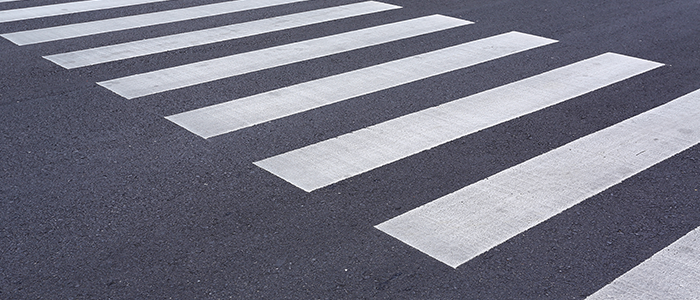
\includegraphics[width=\textwidth]{images/pedestrian.png}
    \end{minipage}
    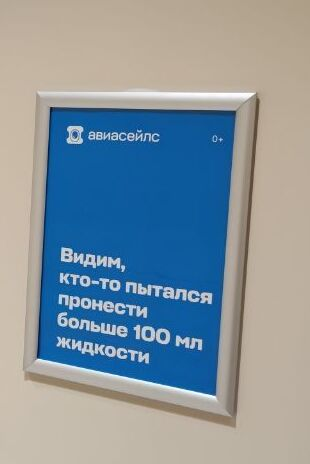
\includegraphics[width=0.3\textwidth]{images/aviasales.png}
    \caption{Исходные изображения}
\end{figure}

\noindent Попробуем применить алгоритм Хафа к этим изображениям. Для этого воспользуемся функцией \texttt{houghlines()} из библиотеки \texttt{OpenCV}. Подберем входные параметры методом тыка и посмотрим на результат.

\begin{figure}[H]
    \centering
    \begin{minipage}{0.48\textwidth}
        \centering
        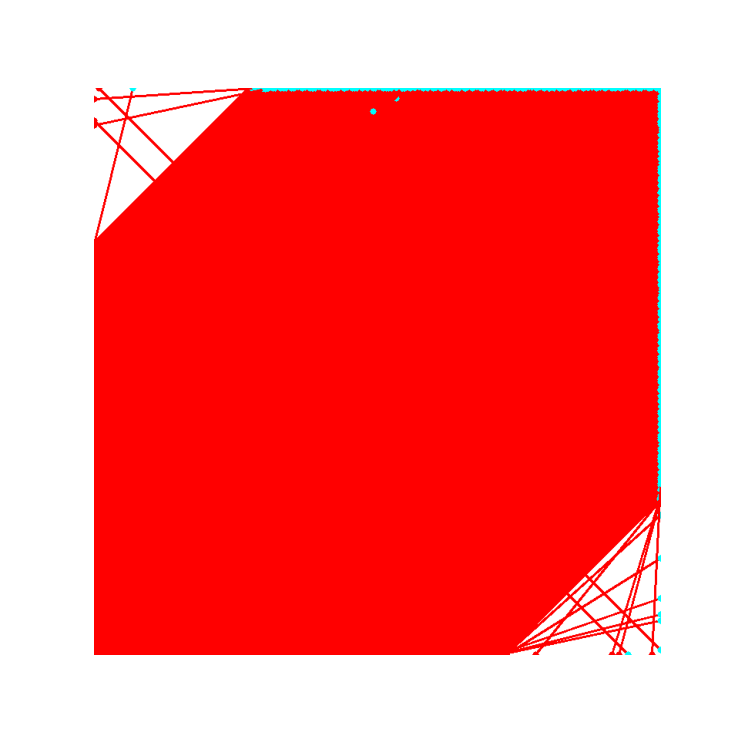
\includegraphics[width=\textwidth]{images/hough_lines/1_orig_hough_lines.png}
    \end{minipage}
    \begin{minipage}{0.48\textwidth}
        \centering
        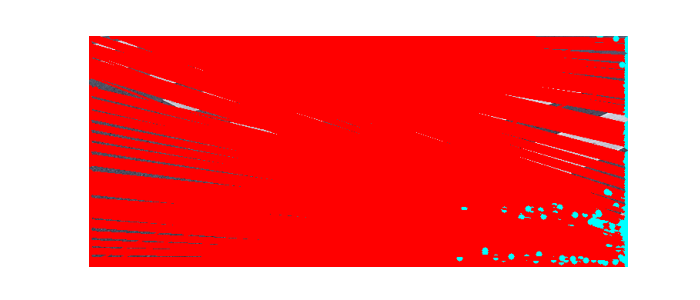
\includegraphics[width=\textwidth]{images/hough_lines/2_orig_hough_lines.png}
    \end{minipage}
    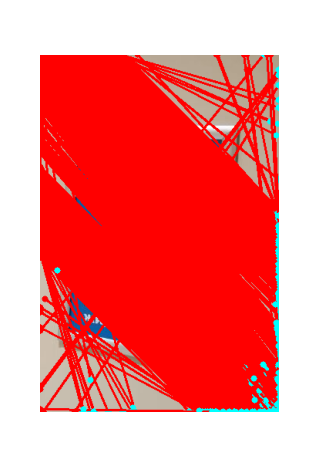
\includegraphics[width=0.3\textwidth]{images/hough_lines/3_orig_hough_lines.png}
    \caption{Алгоритм Хафа на изначальных изображениях}
\end{figure}

\noindent Как мы видим без первоначальной обработки изображений алгоритм Хафа не может найти линии. Попробуем применить к ним фильтры, которые мы изучали в предыдущих лабораторных работах. Для этого воспользуемся функцией \texttt{cv2.GaussianBlur()} и \texttt{cv2.Canny()} из библиотеки \texttt{OpenCV}.

\begin{figure}[H]
    \centering
    \begin{minipage}{0.48\textwidth}
        \centering
        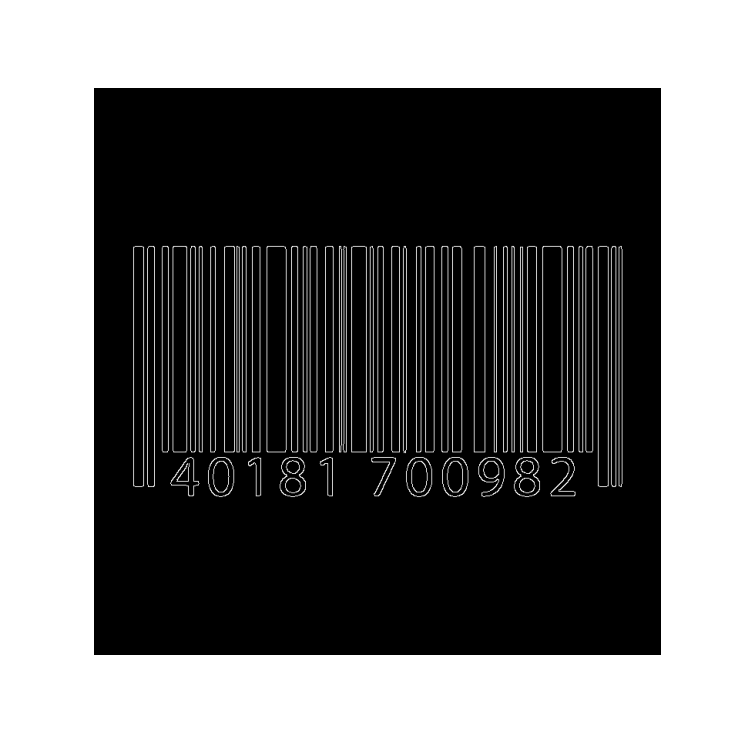
\includegraphics[width=\textwidth]{images/hough_lines/1_proc_canny.png}
    \end{minipage}
    \begin{minipage}{0.48\textwidth}
        \centering
        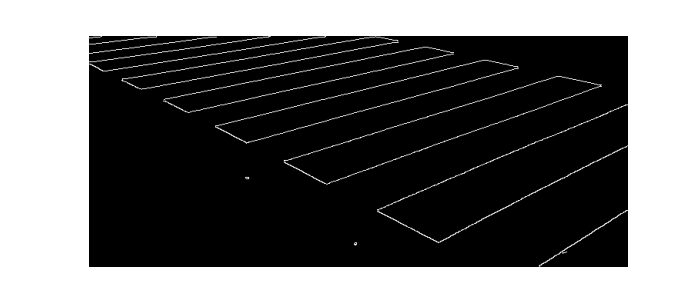
\includegraphics[width=\textwidth]{images/hough_lines/2_proc_canny.png}
    \end{minipage}
    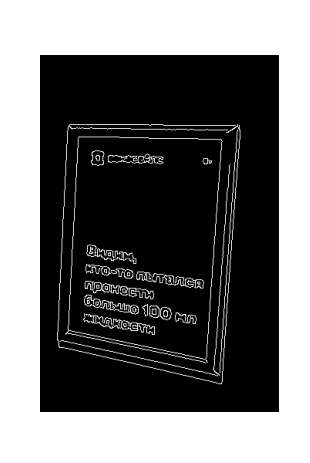
\includegraphics[width=0.3\textwidth]{images/hough_lines/3_proc_canny.png}
    \caption{Изображения, обработанные фильтром Кэнни}
\end{figure}

\noindent Как мы видим, фильтр Кэнни смог выделить контуры на изображении. Теперь попробуем применить алгоритм Хафа к обработанным изображениям и посмотрим на результат.

\begin{figure}[H]
    \centering
    \begin{minipage}{0.48\textwidth}
        \centering
        
\includegraphics[width=\textwidth]{images/hough_lines/1_proc_hough_lines.png}
    \end{minipage}
    \begin{minipage}{0.48\textwidth}
        \centering
        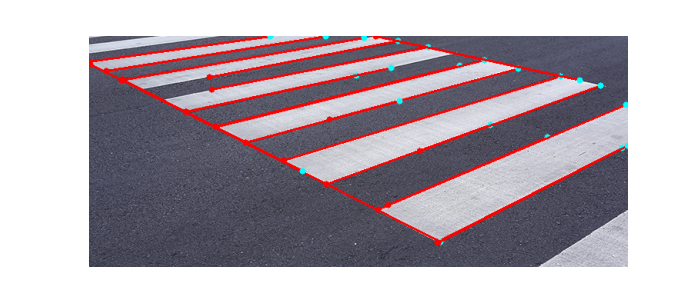
\includegraphics[width=\textwidth]{images/hough_lines/2_proc_hough_lines.png}
    \end{minipage}
    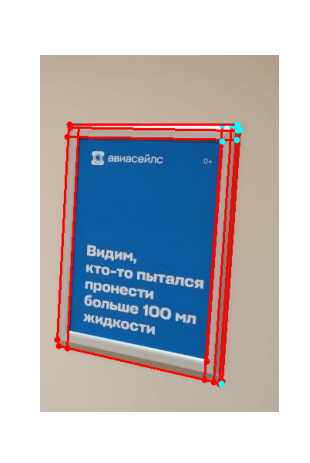
\includegraphics[width=0.3\textwidth]{images/hough_lines/3_proc_hough_lines.png}
    \caption{Алгоритм Хафа на изображениях, обработанных фильтрами}
\end{figure}

\noindent Алгоритм Хафа очень даже хорошо проявил себя в поиске прямых линий. Он корректно нашёл все основные вертикальные полосы на штрихкоде. На пешеходном переходе все полосы «зебры» были выделены как отдельные отрезки, но некоторые края асфальта детектировались фрагментарно из-за разрывов в границах. На постере хорошо выявлены рамочные и крайние угловые линии, но тонкие буквы и мелкая детализация не попадают в результат. 

Теперь построим графики пространств параметров и посмотрим на них.
\begin{figure}[H]
    \centering
    \begin{minipage}{0.48\textwidth}
        \centering
        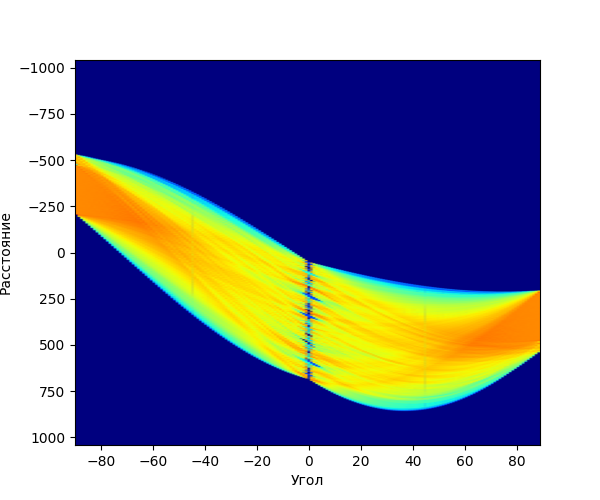
\includegraphics[width=\textwidth]{images/hough_lines/1_proc_accum.png}
    \end{minipage}
    \begin{minipage}{0.48\textwidth}
        \centering
        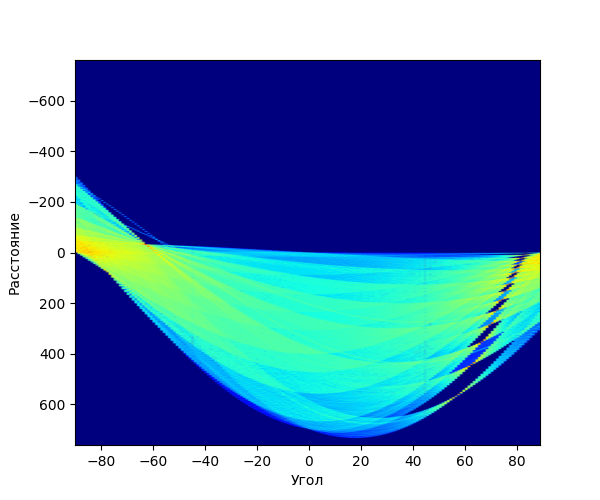
\includegraphics[width=\textwidth]{images/hough_lines/2_proc_accum.png}
    \end{minipage}
    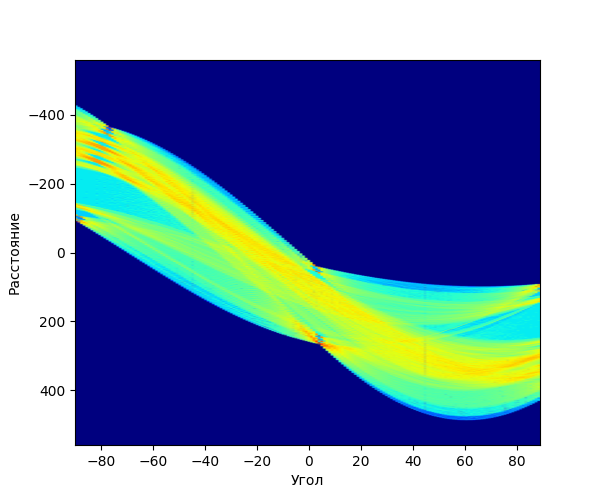
\includegraphics[width=0.48\textwidth]{images/hough_lines/3_proc_accum.png}
    \caption{Графики пространств параметров}
\end{figure}

\noindent На первом графике доминирует яркая вертикальная полоса в центре при $\theta\approx0^\circ$, что соответствует множеству почти вертикальных линий-«штрихов». Белые полосы «зебры» формируют несколько параллельных синусоид, с пиками в районе $\theta\approx0^\circ\pm5^\circ$, что отражает небольшой наклон линий на фото. Основные контуры рамки и наклонённые края плаката дают два множества пиков: один при $\theta\approx-60^\circ$, второй при $\theta\approx70^\circ$. 

Теперь посмотрим на численные результаты. Построим табличку с основной информацией о выявленных линиях.

\begin{table}[h!]
    \centering
    \label{tab:hough-lines}
    \begin{tabular}{c *{3}{r}}
        \textbf{№ изображения} & \textbf{Найдено прямых} & \textbf{Мин. длина, px} & \textbf{Макс. длина, px} \\
        1 & 85 & 254{,}00 & 634{,}00 \\
        2 & 21 & 207{,}16 & 510{,}28 \\
        3 & 11 & 216{,}61 & 334{,}79 \\
    \end{tabular}
    \caption{Результаты поиска прямых линий}
    \end{table}

\paragraph{Выводы:}
\begin{enumerate}
    \item Преобразование Хафа демонстрирует надёжное обнаружение длинных непрерывных прямых участков на изображениях со слабо выраженными шумами.
    \item Параметры HoughLinesP (\texttt{threshold=70}, \texttt{minLineLength=200}, \texttt{maxLineGap=100}) отсекают короткие или слишком прерывистые сегменты. Для обнаружения более коротких или разорванных линий необходимо уменьшать \texttt{minLineLength} или увеличивать \texttt{maxLineGap}.
\end{enumerate}

\section{Поиск окружностей}
В этом разделе попробуем применить алгоритм Хафа для поиска окружностей на изображении. Для этого подготовим изображения, содержащие окружности, и применим к ним преобразование Хафа. Исходные изображения:
\begin{figure}[H]
    \centering
    \begin{minipage}{0.48\textwidth}
        \centering
        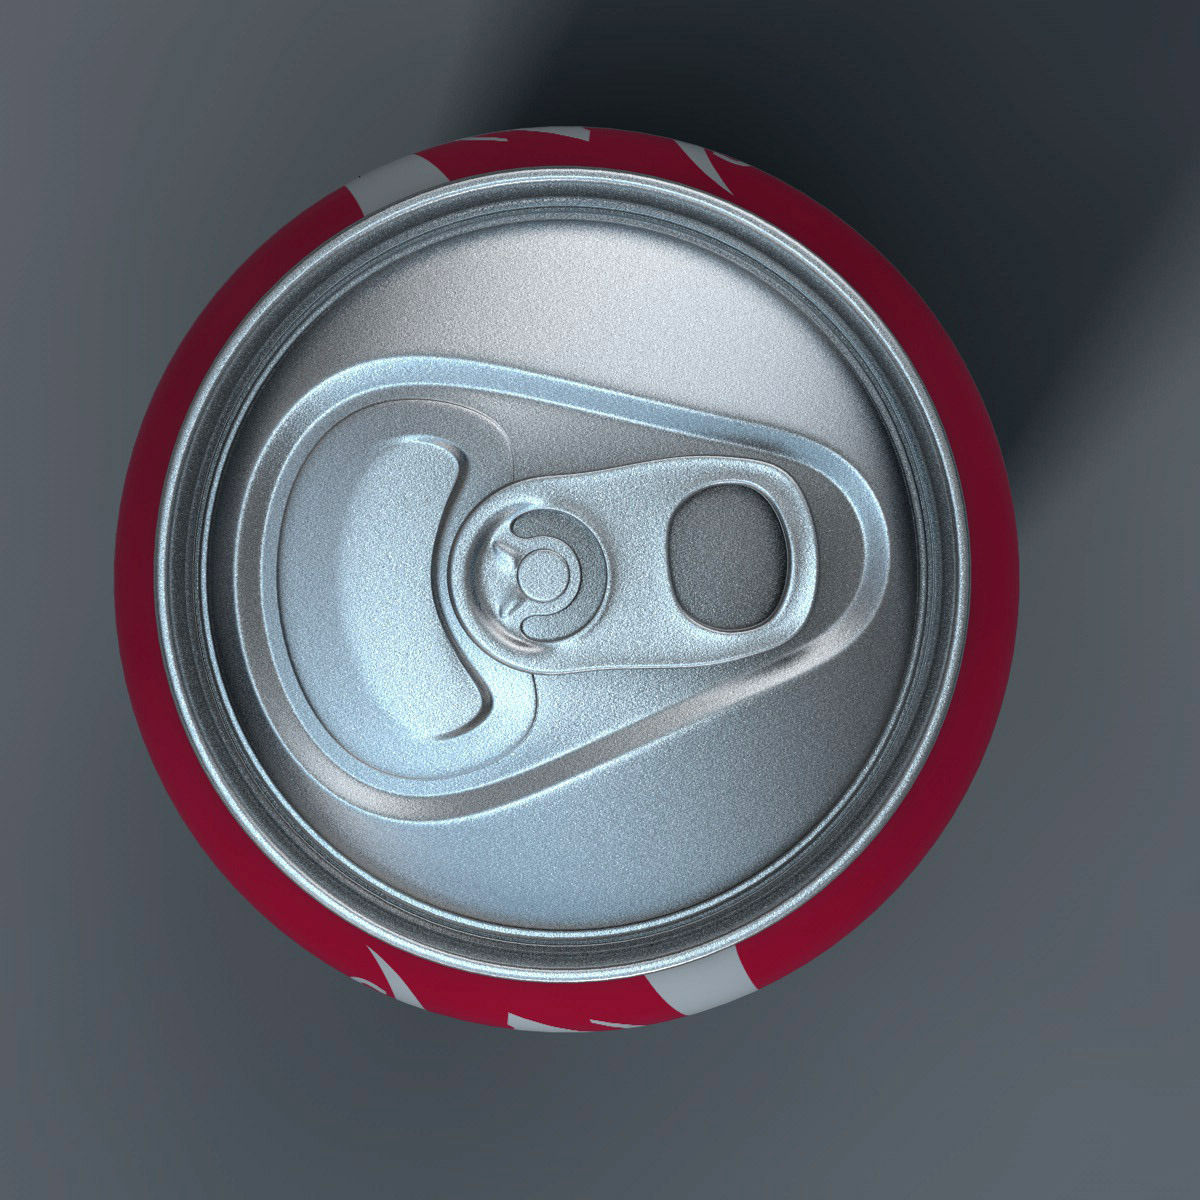
\includegraphics[width=\textwidth]{images/cola.png}
    \end{minipage}
    \begin{minipage}{0.48\textwidth}
        \centering
        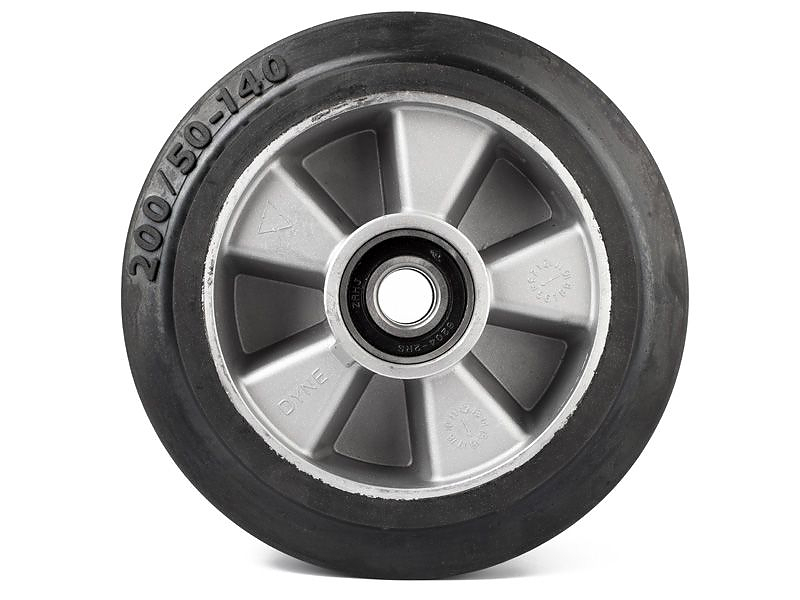
\includegraphics[width=\textwidth]{images/wheel.png}
    \end{minipage}
    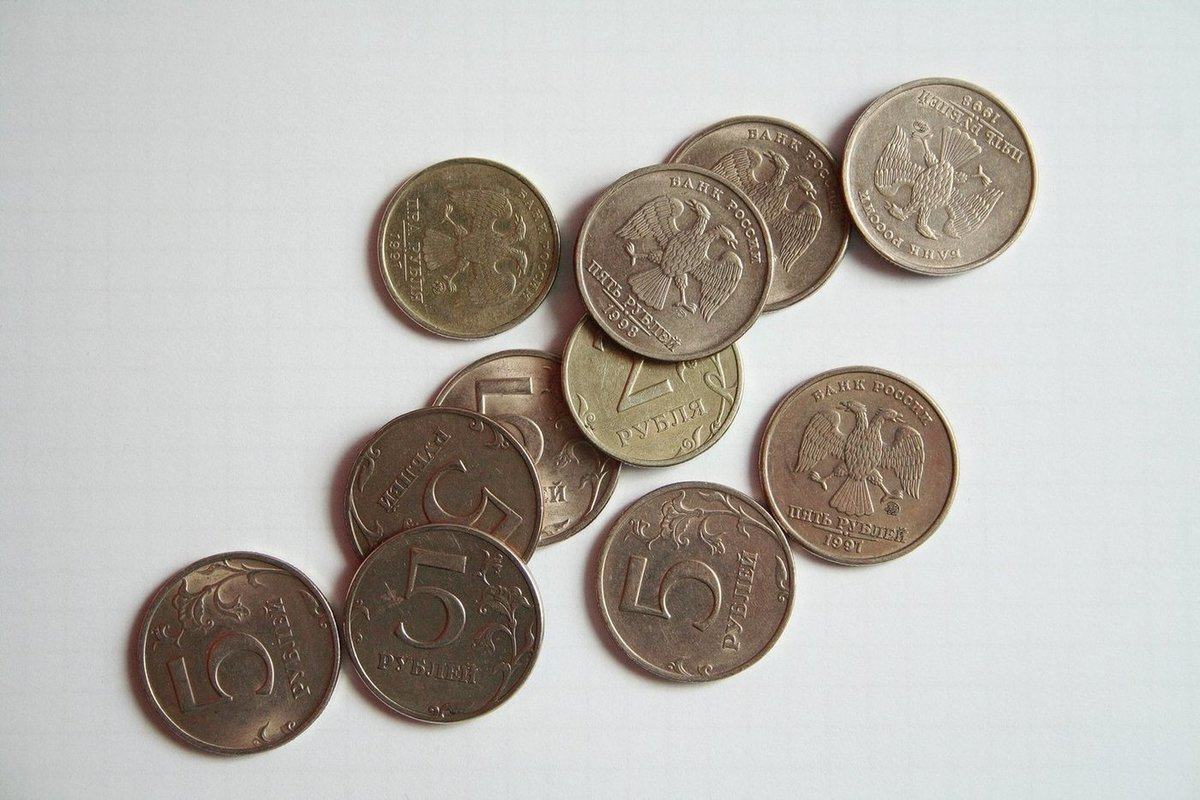
\includegraphics[width=0.48\textwidth]{images/money.png}
    \caption{Исходные изображения}
\end{figure}
Попробуем найти на изображениях окружности определенного радиуса с помощью функции \texttt{cv2.HoughCircles()} из библиотеки \texttt{OpenCV}. Подберем входные параметры методом тыка и посмотрим на результат.
\begin{figure}[H]
    \centering
    \begin{minipage}{0.48\textwidth}
        \centering
        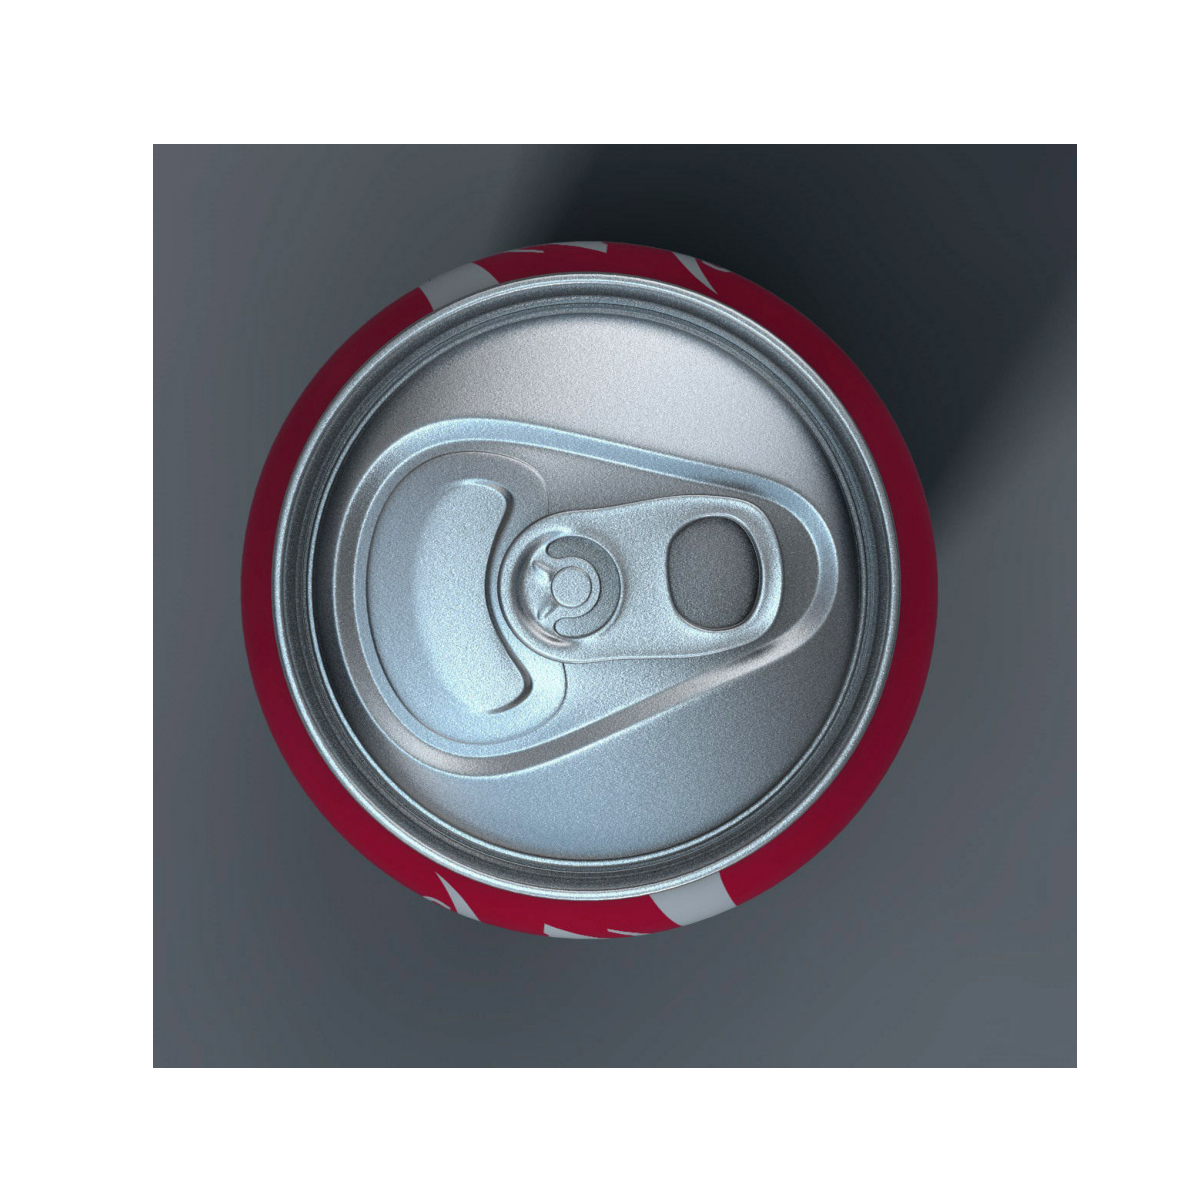
\includegraphics[width=\textwidth]{images/hough_circles/1_orig_fixed.png}
    \end{minipage}
    \begin{minipage}{0.48\textwidth}
        \centering
        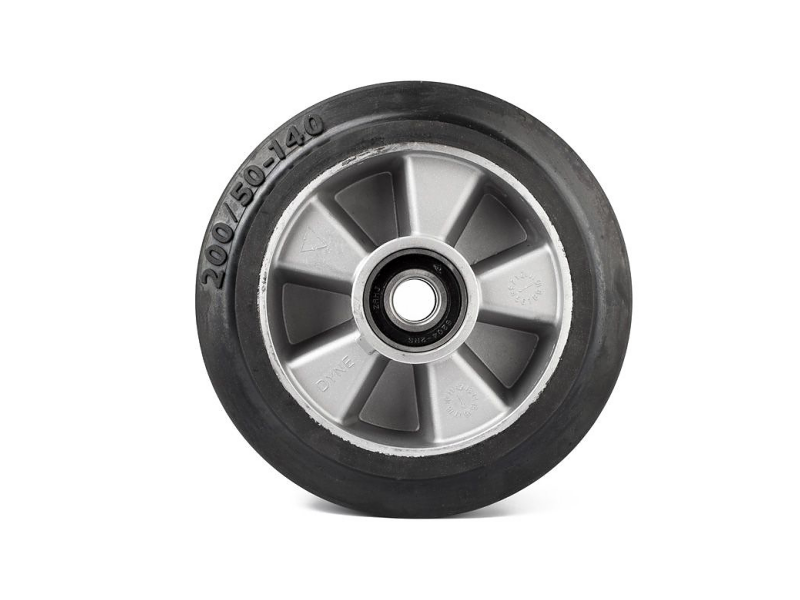
\includegraphics[width=\textwidth]{images/hough_circles/3_orig_fixed.png}
    \end{minipage}
    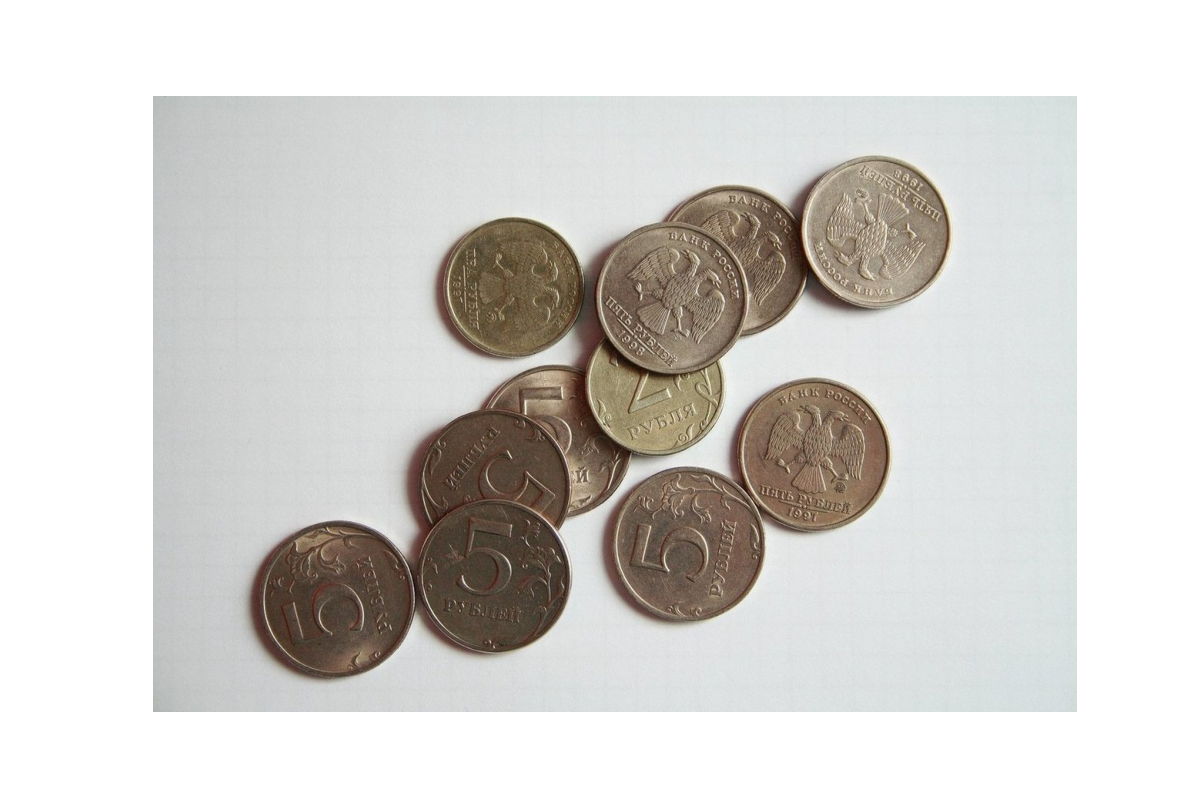
\includegraphics[width=0.48\textwidth]{images/hough_circles/2_orig_fixed.png}
    \caption{Алгоритм Хафа на изначальных изображениях, поиск фиксированного радиуса}
\end{figure}
\noindent Как мы видим, алгоритм Хафа не может найти окружности. Все потому что мы задали жесткие ограничения на радиус окружностей при поиске. Попробуем найти окружности с переменным радиусом окружностей.
\begin{figure}[H]
    \centering
    \begin{minipage}{0.48\textwidth}
        \centering
        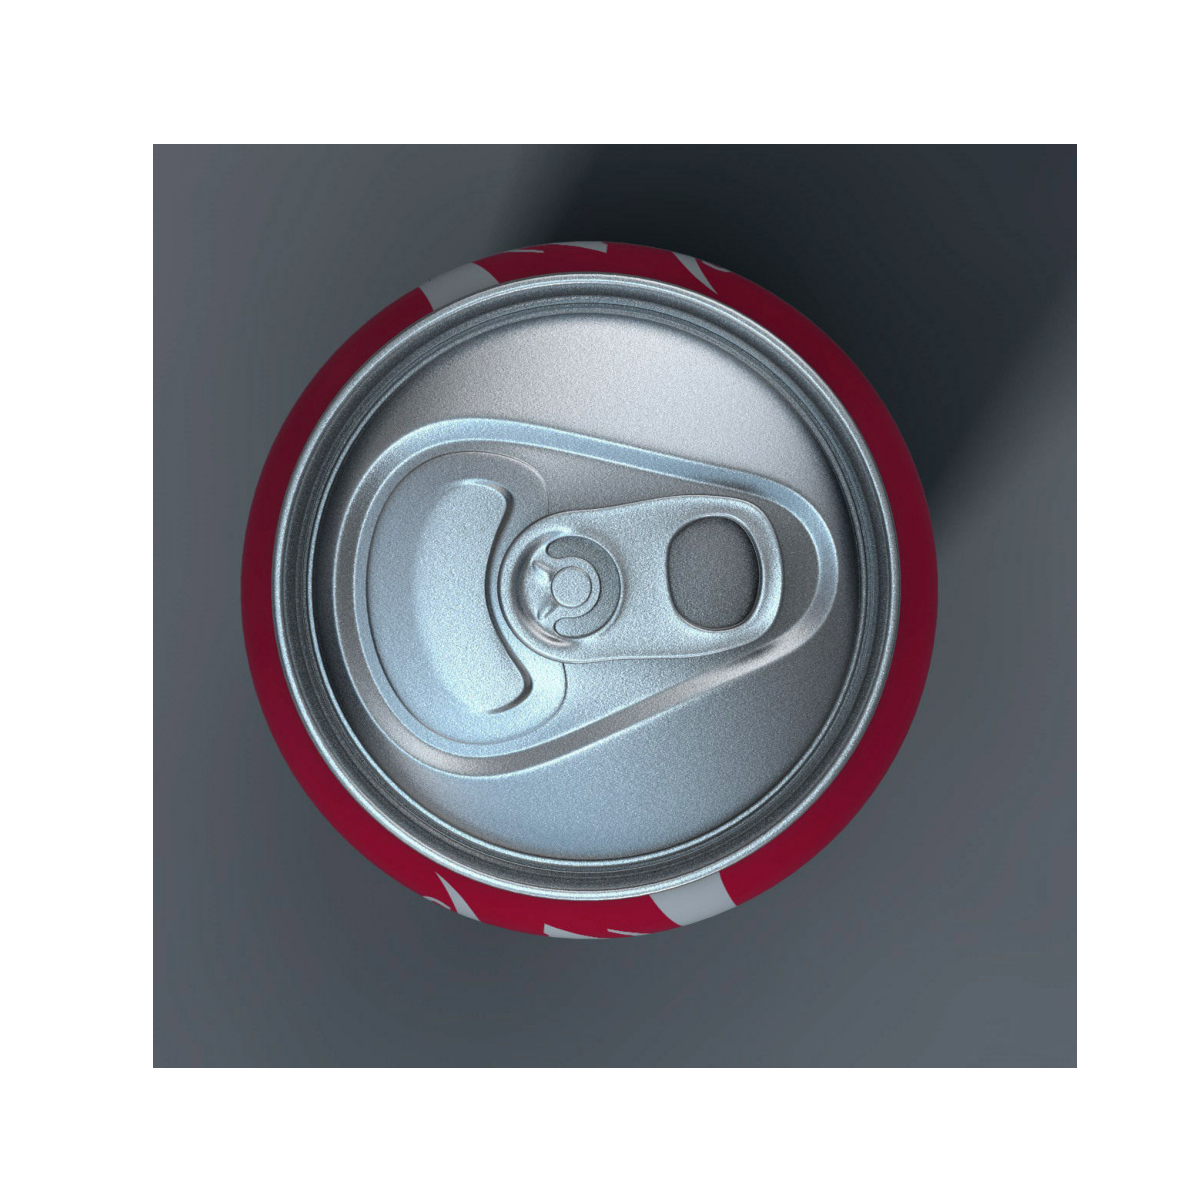
\includegraphics[width=\textwidth]{images/hough_circles/1_orig_range.png}
    \end{minipage}
    \begin{minipage}{0.48\textwidth}
        \centering
        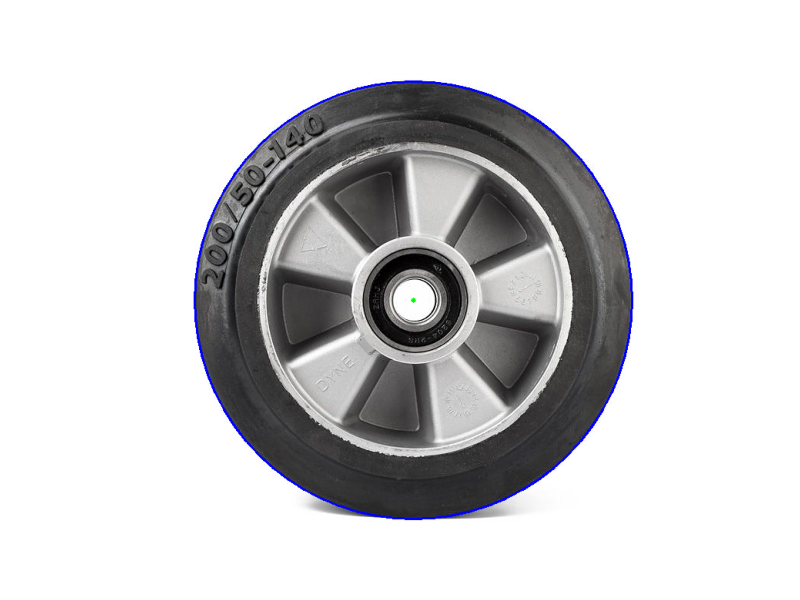
\includegraphics[width=\textwidth]{images/hough_circles/3_orig_range.png}
    \end{minipage}
    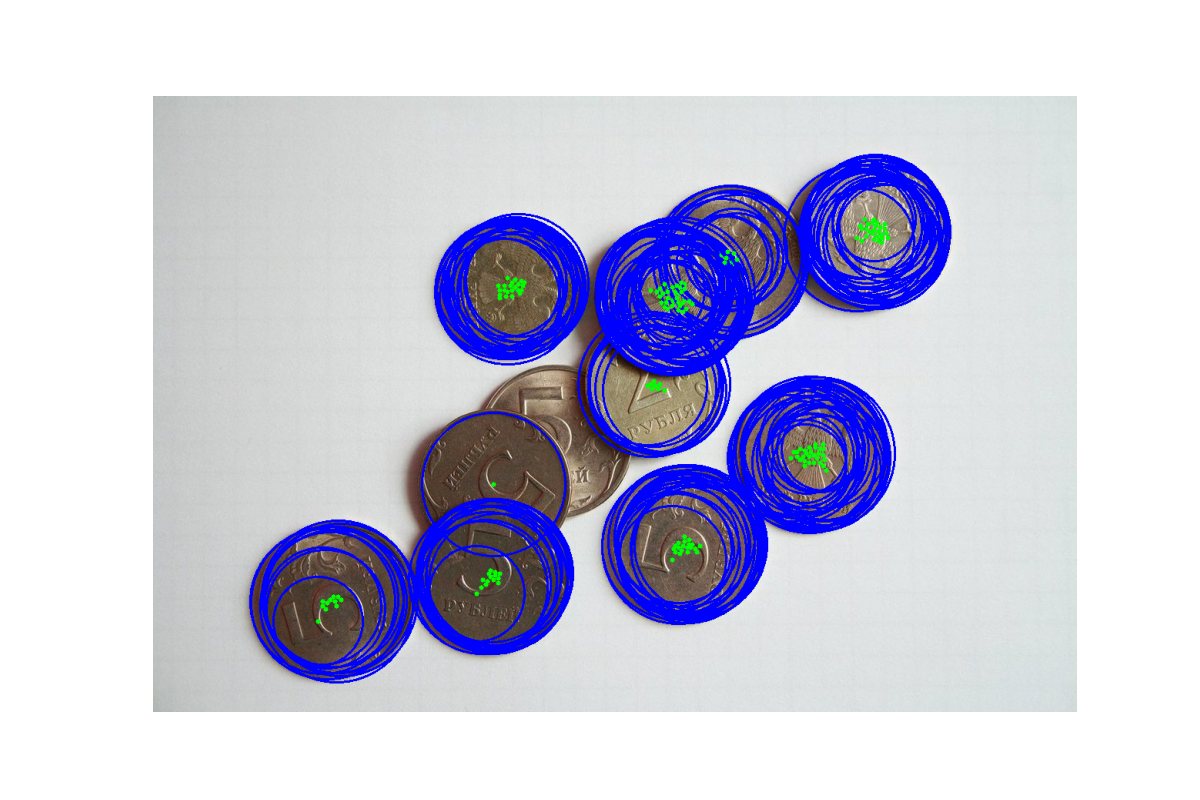
\includegraphics[width=0.48\textwidth]{images/hough_circles/2_orig_range.png}
    \caption{Алгоритм Хафа на изначальных изображениях, поиск радиуса в некотором диапазоне}
\end{figure}

\noindent Как мы видим, алгоритм Хафа смог найти окружности на 2 изображениях из 3. Но на 2 изображении видно, что алгоритм выделил большое количество окружностей, а это усложняет поиск истинного контура. С колесом ситуация лучше, но алгоритм не увидел окружности внутри колеса. Теперь попробуем применить к ним фильтры: \texttt{cv2.GaussianBlur()} и \texttt{cv2.Canny()}. Посмотрим на результат.
\begin{figure}[H]
    \centering
    \begin{minipage}{0.48\textwidth}
        \centering
        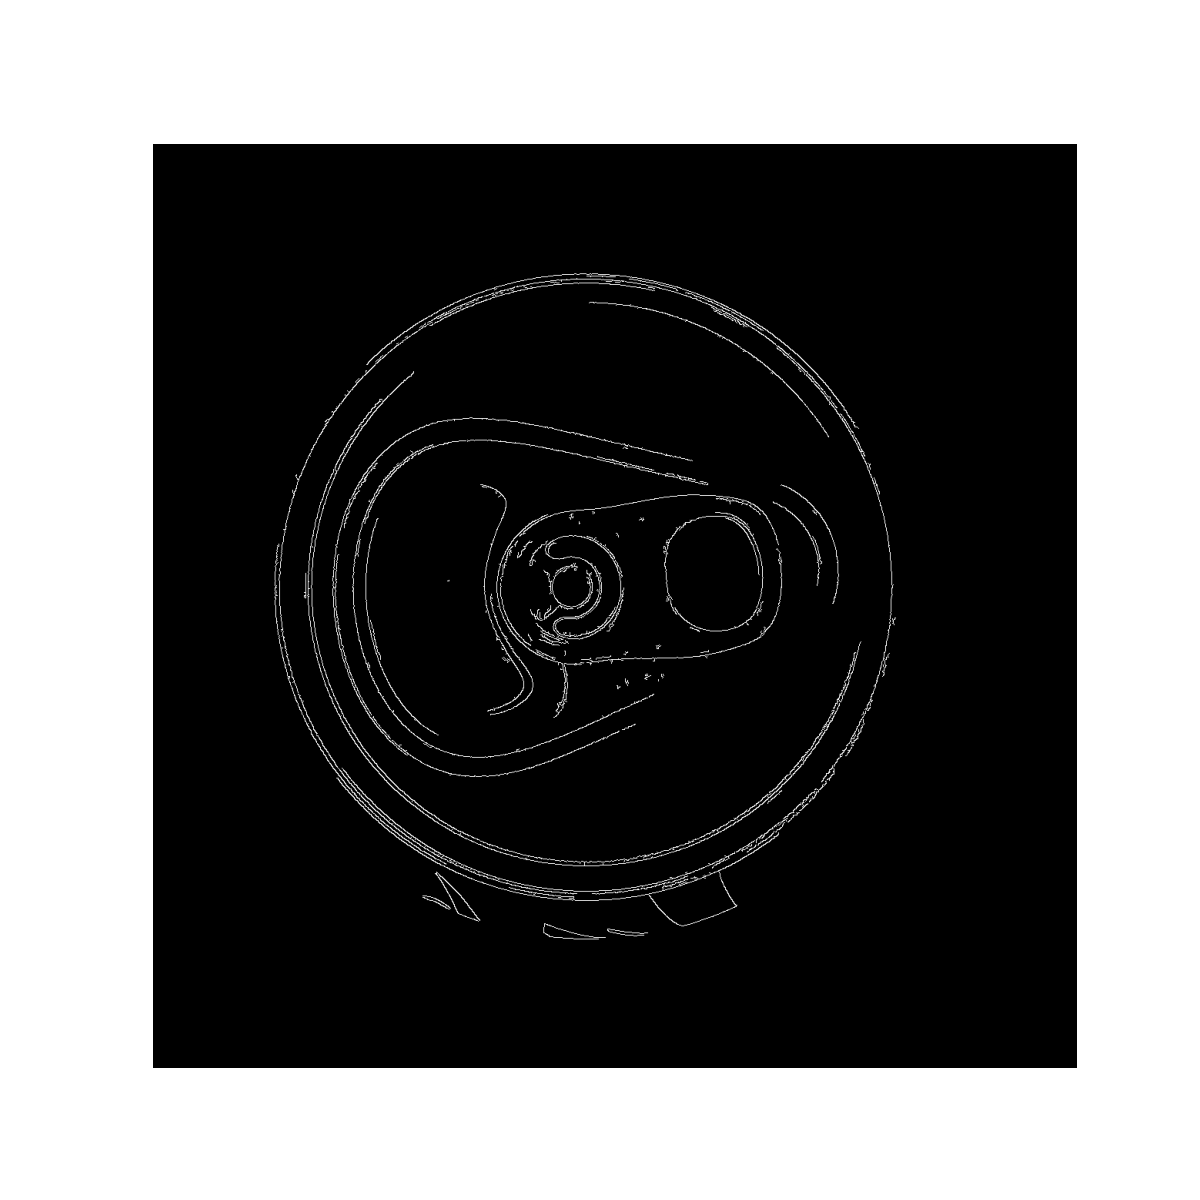
\includegraphics[width=\textwidth]{images/hough_circles/1_proc_canny.png}
    \end{minipage}
    \begin{minipage}{0.48\textwidth}
        \centering
        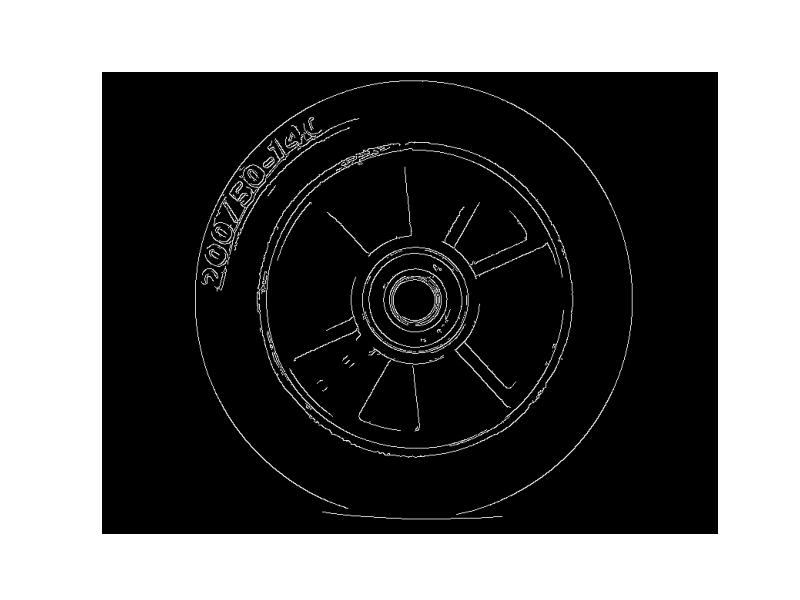
\includegraphics[width=\textwidth]{images/hough_circles/3_proc_canny.png}
    \end{minipage}
    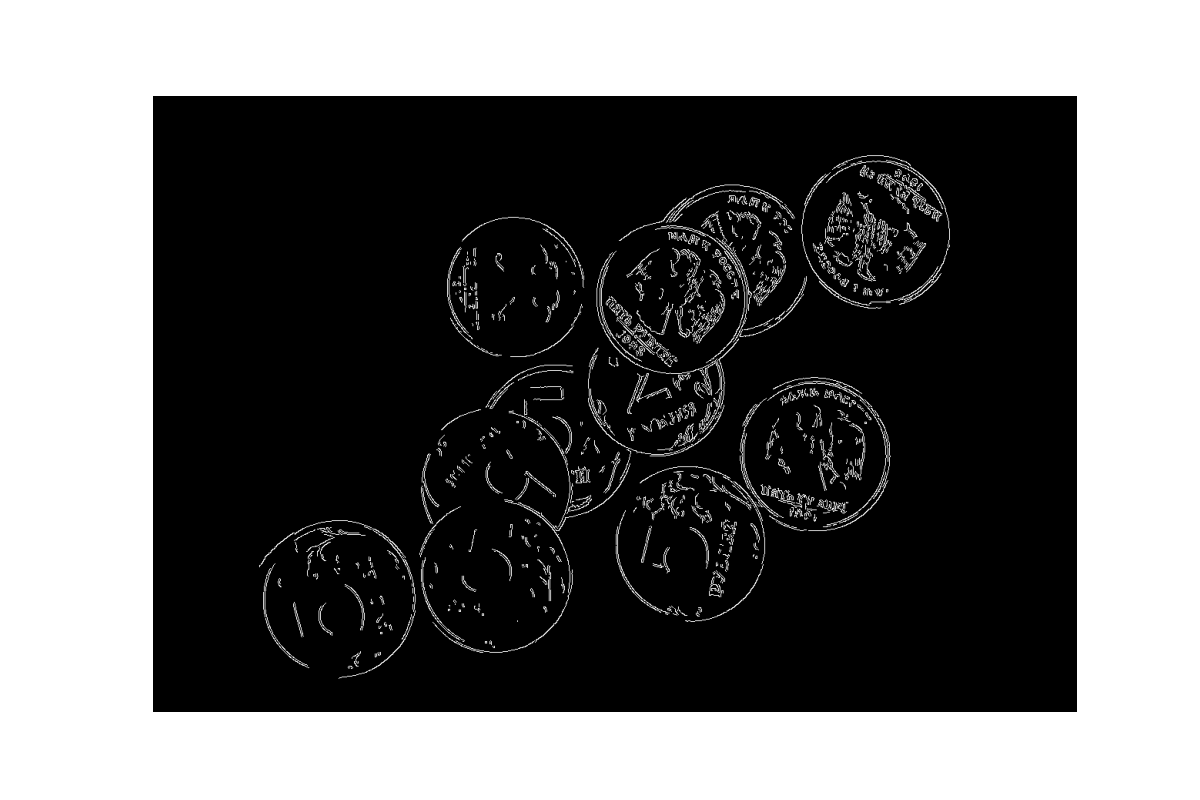
\includegraphics[width=0.48\textwidth]{images/hough_circles/2_proc_canny.png}
    \caption{Изображения, обработанные фильтром Кэнни}
\end{figure}
\noindent Как мы видим, фильтр Кэнни сделал контуры более выраженными. Теперь попробуем применить алгоритм Хафа к обработанным изображениям и посмотрим на результат.

\begin{figure}[H]
    \centering
    \begin{minipage}{0.48\textwidth}
        \centering
        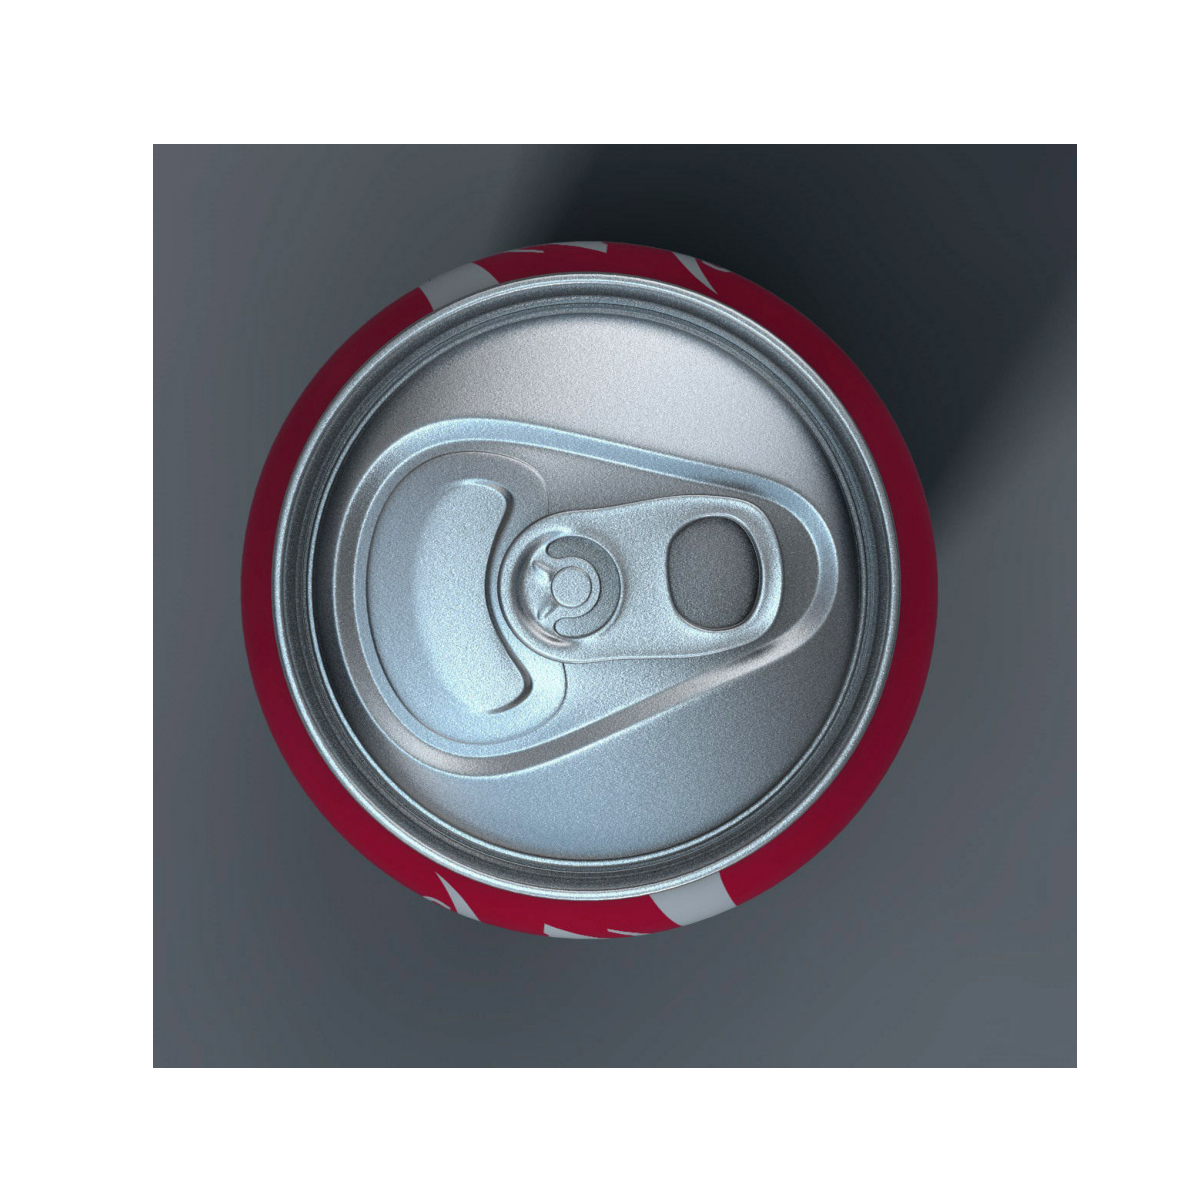
\includegraphics[width=\textwidth]{images/hough_circles/1_proc_fixed.png}
    \end{minipage}
    \begin{minipage}{0.48\textwidth}
        \centering
        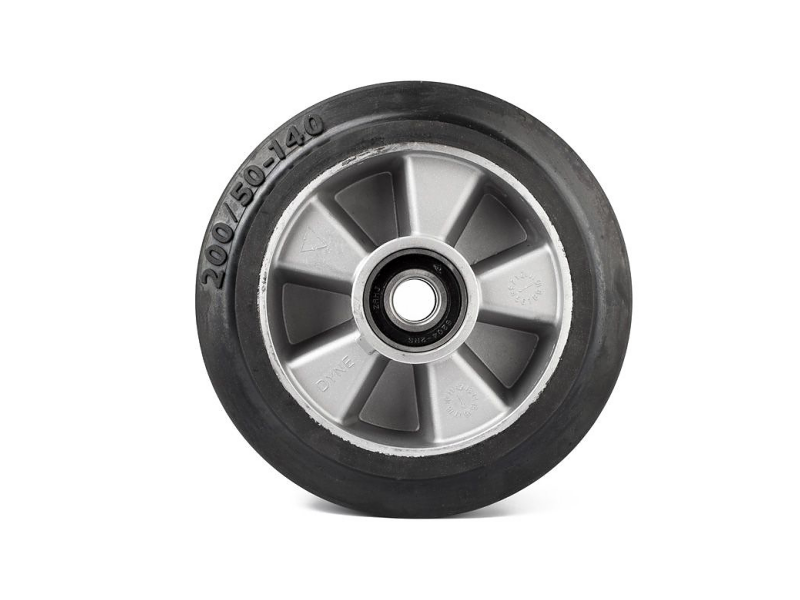
\includegraphics[width=\textwidth]{images/hough_circles/3_proc_fixed.png}
    \end{minipage}
    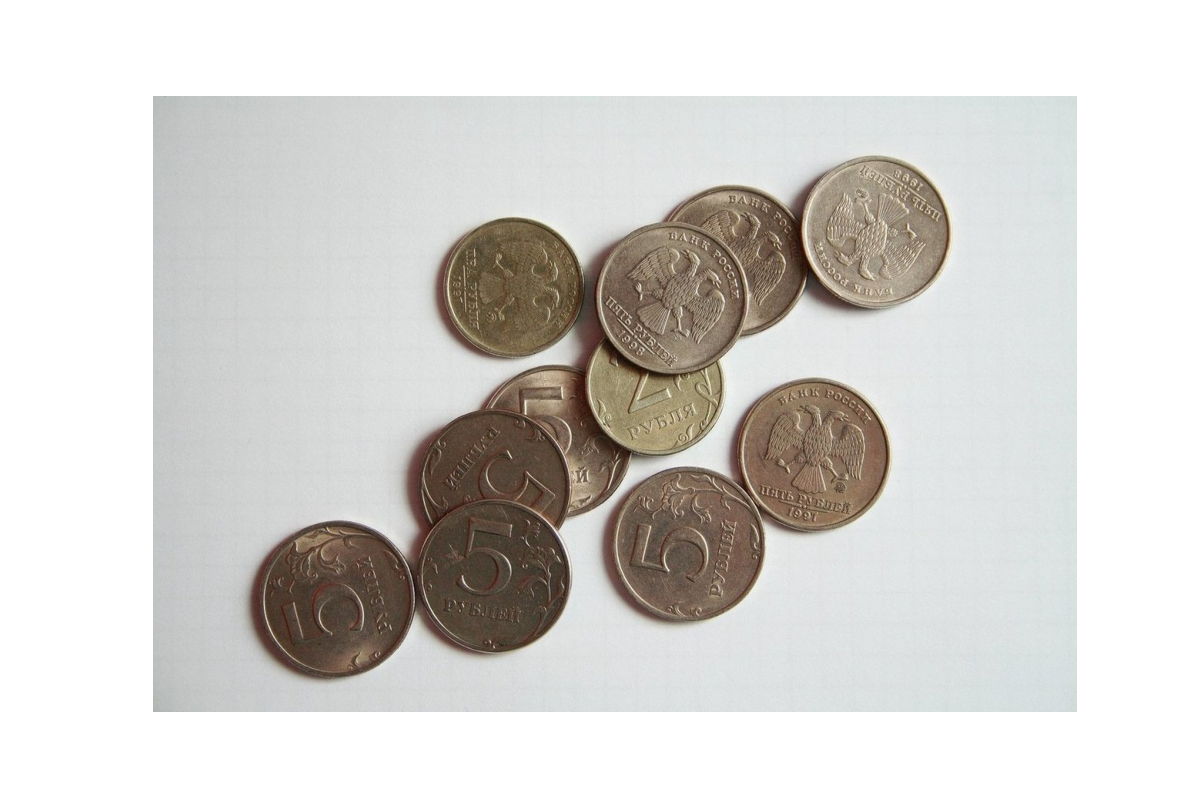
\includegraphics[width=0.48\textwidth]{images/hough_circles/2_proc_fixed.png}
    \caption{Алгоритм Хафа на изображениях, обработанных фильтрами, поиск фиксированного радиуса}
\end{figure}
\noindent Как и предпалагалось задать точный радиус сложно, поэтому алгоритм не находит окружностей. Попробуем найти окружности с переменным радиусом. 
\begin{figure}[H]
    \centering
    \begin{minipage}{0.48\textwidth}
        \centering
        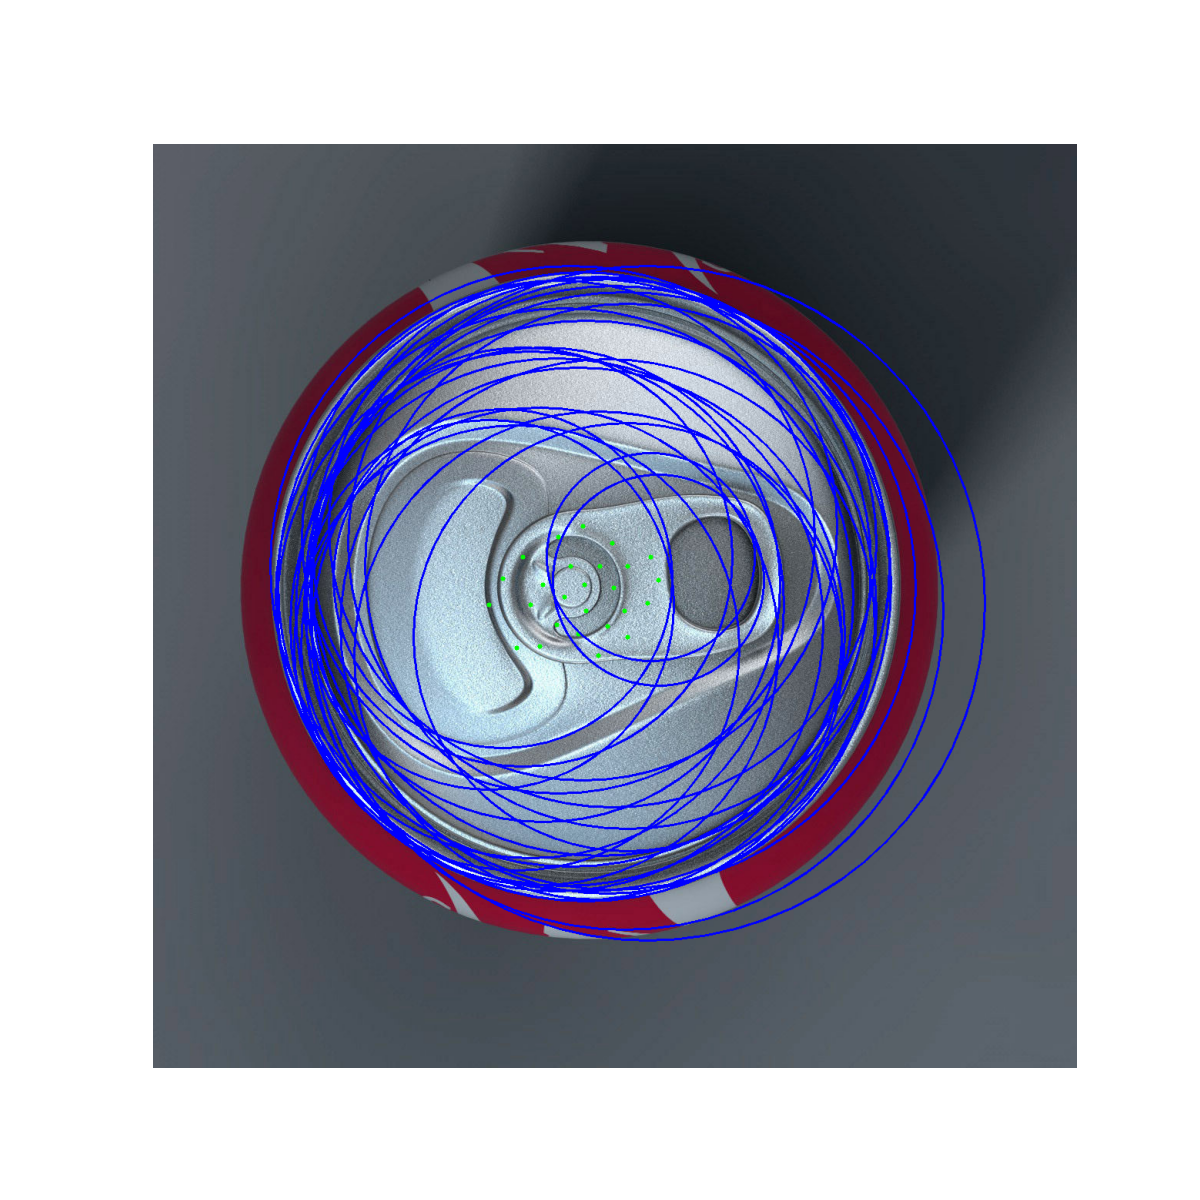
\includegraphics[width=\textwidth]{images/hough_circles/1_proc_range.png}
    \end{minipage}
    \begin{minipage}{0.48\textwidth}
        \centering
        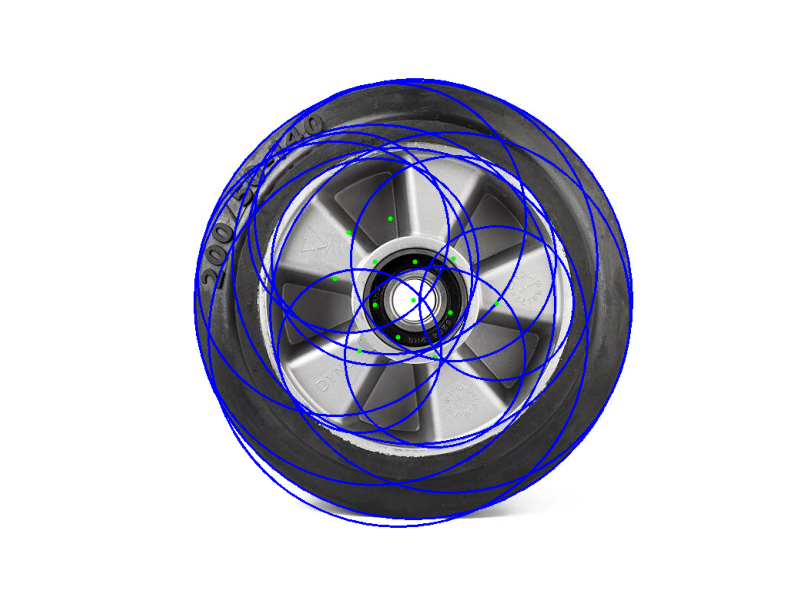
\includegraphics[width=\textwidth]{images/hough_circles/3_proc_range.png}
    \end{minipage}
    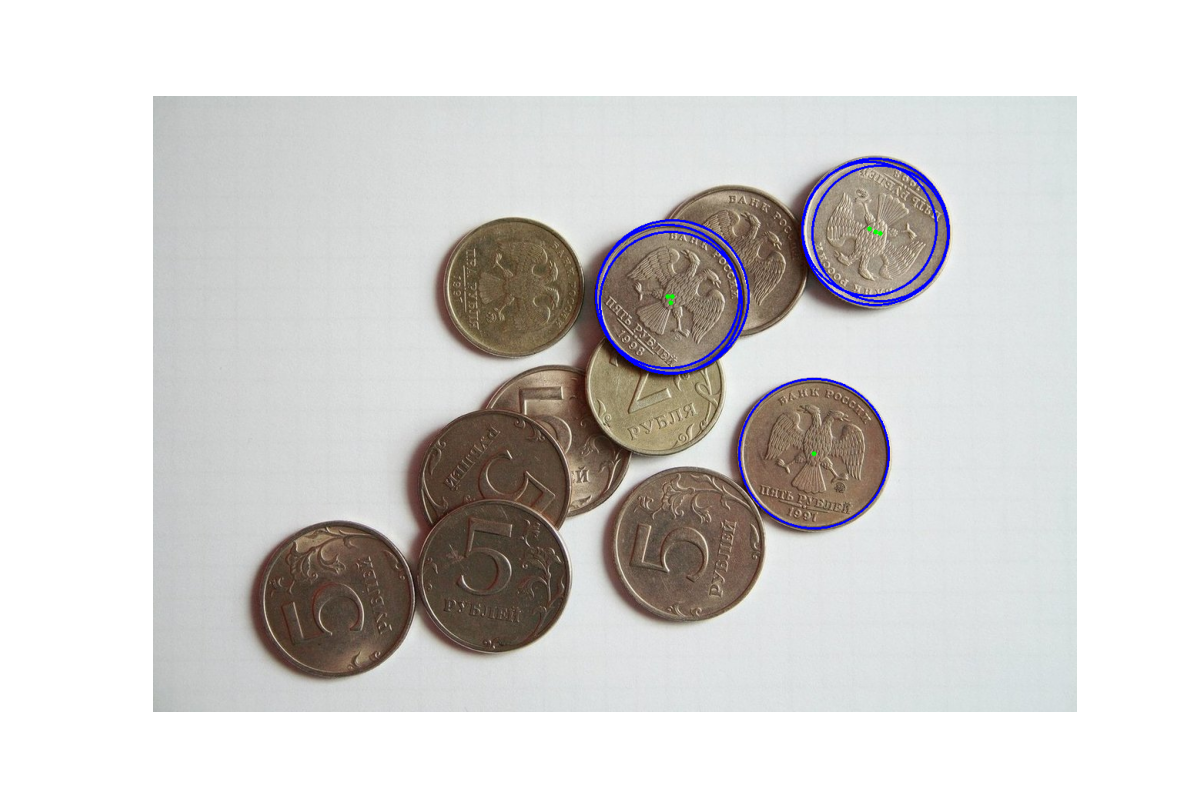
\includegraphics[width=0.48\textwidth]{images/hough_circles/2_proc_range.png}
    \caption{Алгоритм Хафа на изображениях, обработанных фильтрами, поиск радиуса в некотором диапазоне}
\end{figure}
\noindent Как мы видим, алгоритм Хафа смог найти окружности на всех изображениях. На первом было обнаружено множество круговых контуров крышки от банки, в том числе внутренние детали, что привело к большинству ложных окружностей. На втором изображении алгоритм выделил меньше монет, но более точно, по сравнению с тем, что было до применения фильтра. Диапазон радиусов был удачно подобран под диаметр монет, благодаря чему алгоритм корректно выделил 3 монеты. 

На третьем изображении алгоритм выделил множество окружностей, но не все из них соответствуют истинным кругам. По внешнему и центральному ободам диска окружности определяются чётко. Тем не менее возможно диск и протектор шины дают ложные круги. 
\paragraph{Выводы:}
\begin{itemize}
    \item Точный подбор \texttt{minRadius}/\texttt{maxRadius} критически важен: широкий диапазон даёт ложные окружности, узкий --- пропускает объекты.
    \item Рекомендуется сортировать найденные окружности по метрике и удалять близкие дубли по центру для повышения точности.
    \item Преобразование Хафа демонстрирует возможность обнаружения окружностей на изображениях, но требует тщательной подготовки изображений и настройки параметров.
\end{itemize}

\section{Вывод}
В ходе выполнения лабораторной работы были реализованы и исследованы два классических применения преобразования Хафа:

\begin{enumerate}
  \item Поиск прямых линий на трёх произвольных изображениях:
    \begin{itemize}
      \item Выделение границ методом Canny позволило получить чёткую бинарную маску контуров.
      \item Алгоритм Хафа надёжно детектировал главные линейные элементы (штрихи, дорожную разметку, контурные кромки).
      \item Было обнаружено от 11 до 85 прямых на разных изображениях; минимальная длина отрезков варьировалась в пределах от 150 до 254px, максимальная --- 334–634px.
    \end{itemize}

  \item Поиск окружностей на трёх произвольных изображениях:
    \begin{itemize}
      \item Gaussian Blur сглаживал шум, Canny подчёркивал контуры, но вместе они могли генерировать ложные отклики от рельефа.
      \item Для монет алгоритм успешно нашёл основные окружности, но не все.
      \item В случаях баночной крышки и автомобильного диска множество мелких деталей (резьба, спицы) дало ложные круги, что требует дополнительной фильтрации по метрикеи удалению дублирующих кандидатов.
    \end{itemize}
\end{enumerate}

\section{Вопросы к защите}
\begin{enumerate}
    \item \textbf{Какая идея лежит в основе преобразования Хафа?}\\[0.3em]
    Каждая точка контура на изображении «голосует» за все возможные примитивы (прямые, окружности и т.\,д.), которые могут через неё проходить. В пространстве параметров аккумулируются эти голоса, и локальные максимумы аккумуляторной функции соответствуют наиболее вероятным геометрическим объектам в исходном изображении.

    \item \textbf{Можно ли использовать преобразование Хафа для поиска произвольных контуров, которые невозможно описать аналитически?}\\[0.3em]
    Да. Для этого применяется \emph{обобщённое преобразование Хафа}. Вместо явного параметрического уравнения используется R-таблица — набор векторных смещений от точек эталонного контура к его «центру». Каждая точка изображения голосует по этой таблице, что позволяет обнаруживать объекты сложной формы.

    \item \textbf{Что такое рекуррентное и обобщённое преобразования Хафа?} \\[0.3em]
    \emph{Обобщённое преобразование Хафа} — метод, в котором шаблонная форма хранится в виде R-таблицы, и по ней голосуют точки изображения за все возможные положения контура.\\
    \emph{Рекуррентное преобразование Хафа} — многоступенчатый подход: после обнаружения сильнейших примитивов их голоса обнуляются, и алгоритм повторно запускается для выявления менее выраженных объектов.
    \item \textbf{Какие бывают способы параметризации в преобразовании Хафа?} \\[0.3em]
    Можно выделить несколько способов параметризации:
    \begin{itemize}
        \item Для прямых:
          \begin{enumerate}
            \item Наклонно‑пересечная форма: \(y = kx + b\).
            \item Нормальная форма: \(x\cos\Theta + y\sin\Theta = \rho\).
          \end{enumerate}
        \item Для окружностей: \((x - x_0)^2 + (y - y_0)^2 = R^2\) с параметрами \((x_0,y_0,R)\).
        \item Для эллипсов, парабол и других кривых используются соответствующие параметрические уравнения (набор коэффициентов \(a_1,\dots,a_n\)).
        \item В обобщённом Хафа — таблица, задающая смещения от контура к его центру.
      \end{itemize}
\end{enumerate}
\end{document}
